\documentclass[../main.tex]{subfiles}

\graphicspath{{\subfix{../figures/}}}

\begin{document}
Many datasets obtained through \gls{cryoem} demonstrate heterogeneity, indicating that a single 3D structure cannot be attributed to the acquisition. Two potential reasons account for this diversity. Firstly, the studied specimen might exhibit flexibility, resulting in projections originating from distinct protein states. This  phenomenon is referred as conformational heterogeneity. Secondly, the images may involve a drug binding experiment, with some projections feature a small attached drug while others do not. This last case is known as compositional heterogeneity.

Regardless of the heterogeneity type, 2D projections need to be categorized according to the 3D structure they belong to, so that each of the classes can be used to reconstruct a disctinct volume homogeneously. This projection classification problem is known as 3D classification. The main difficulty of this process is that the actual variations in the structures are not known. In other words, images need to be segregated according to a criteria that it is not known yet, implying that the partition must be data-driven. This is further hampered by the fact that variations between structures are very subtle and the signal to noise ratio in the data is extremely low. The process is illustrated in Figure \ref{fig:1.1:3d_classification}.

\begin{figure}[hbp]
    \centering
    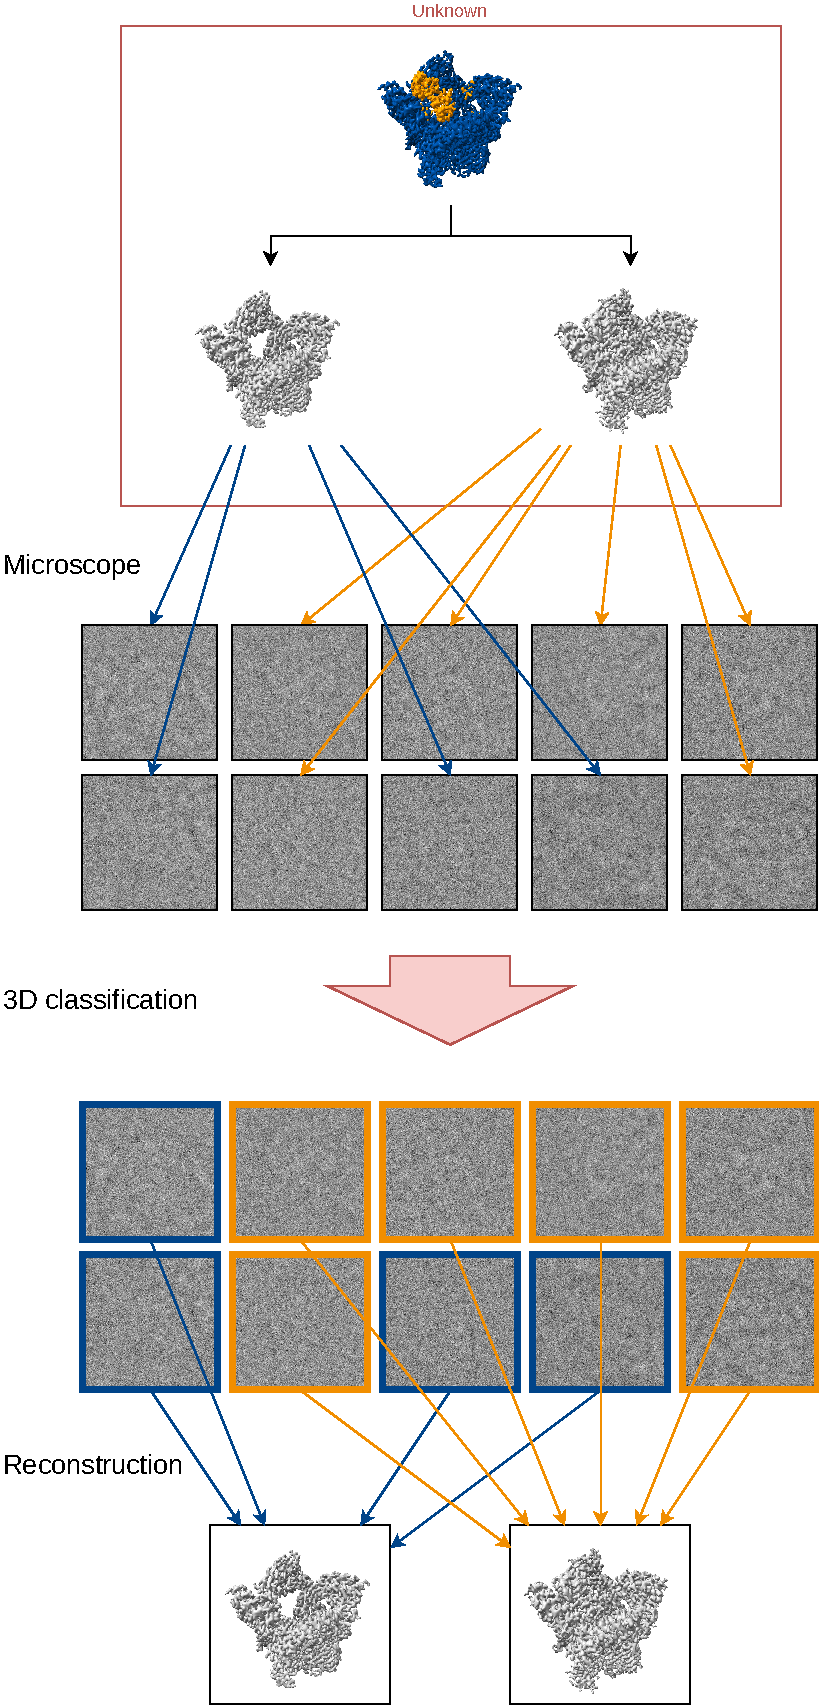
\includegraphics[width=.65\textwidth]{3D classification}
    \caption{Example of a 3D classification}
    \label{fig:1.1:3d_classification}
\end{figure}

Nevertheless, the 3D classification step is provided with some ancillary parameter estimations. For instance, the projection parameters have been estimated by the previous steps in the image processing pipeline. With these parameters, a mixture of the unknown structures can be reconstructed, known as ``consensus volume''.

\end{document}
 
